\section{An Attack to the Shared Entities Contract}\label{sec:attack}

Let us state an important property about shared entities:
%
\vspace{2ex}
\begin{mdframed}[leftmargin=10pt,rightmargin=10pt]
  \begin{center}\emph{Consistency of Shareholders}\end{center}
  \noindent
  If \<se> is a {\codesize\texttt{SharedEntity<S,O>}}
  then \<se.getShareholders()> contains only elements of type \<S>.
\end{mdframed}
\vspace{2ex}
%
This property is important since it states that one can trust the type \<S> of
the shareholders: if one creates a \<SharedEntity> and fixes a specific type \<S>
for its shareholders, then only instances of \<S> will actually manage to become shareholders.

It turns out that the \emph{Consistency of Shareholders} property holds
for instances of the class \<SimpleSharedEntity> in Fig.~\ref{fig:simple_shared_entity}.
Namely, that class does not use unchecked casts, hence it is strongly-typed~\cite{NaftalinW06} and
its map \<shares> actually holds values of type \<S> in its domain, only.
For this consistency result, one needs
the dummy \<buyer> argument for the method \<accept>
of the shared entities. Without that argument, the
\emph{Consistency of Shareholders} property would not hold, since one could only write
\<addShares((S) caller(), offer.sharesOnSale)> in the implementation of \<accept> in
Fig.~\ref{fig:simple_shared_entity}, with an unchecked cast that makes its code
non-strongly-typed. In that case, also contracts not of type \<S> could call \<accept>
and become shareholders.

\begin{figure}[ht]
  \begin{center}
    \begin{lstlisting}[language=Takamaka]
public class Attacker extends ExternallyOwnedAccount {

  public Validator(String publicKey) {
    super(publicKey);
  }

  @View
  public String id() {
    return /* id of the victim blockchain node, unrelated to publicKey */
  }
}
    \end{lstlisting}
  \end{center}
  \caption{An attacker that exploits the work of a blockchain validator node and fraudolently earns the rewards of that work.}\label{fig:attacker}
\end{figure}

\begin{figure*}[ht]
\centering
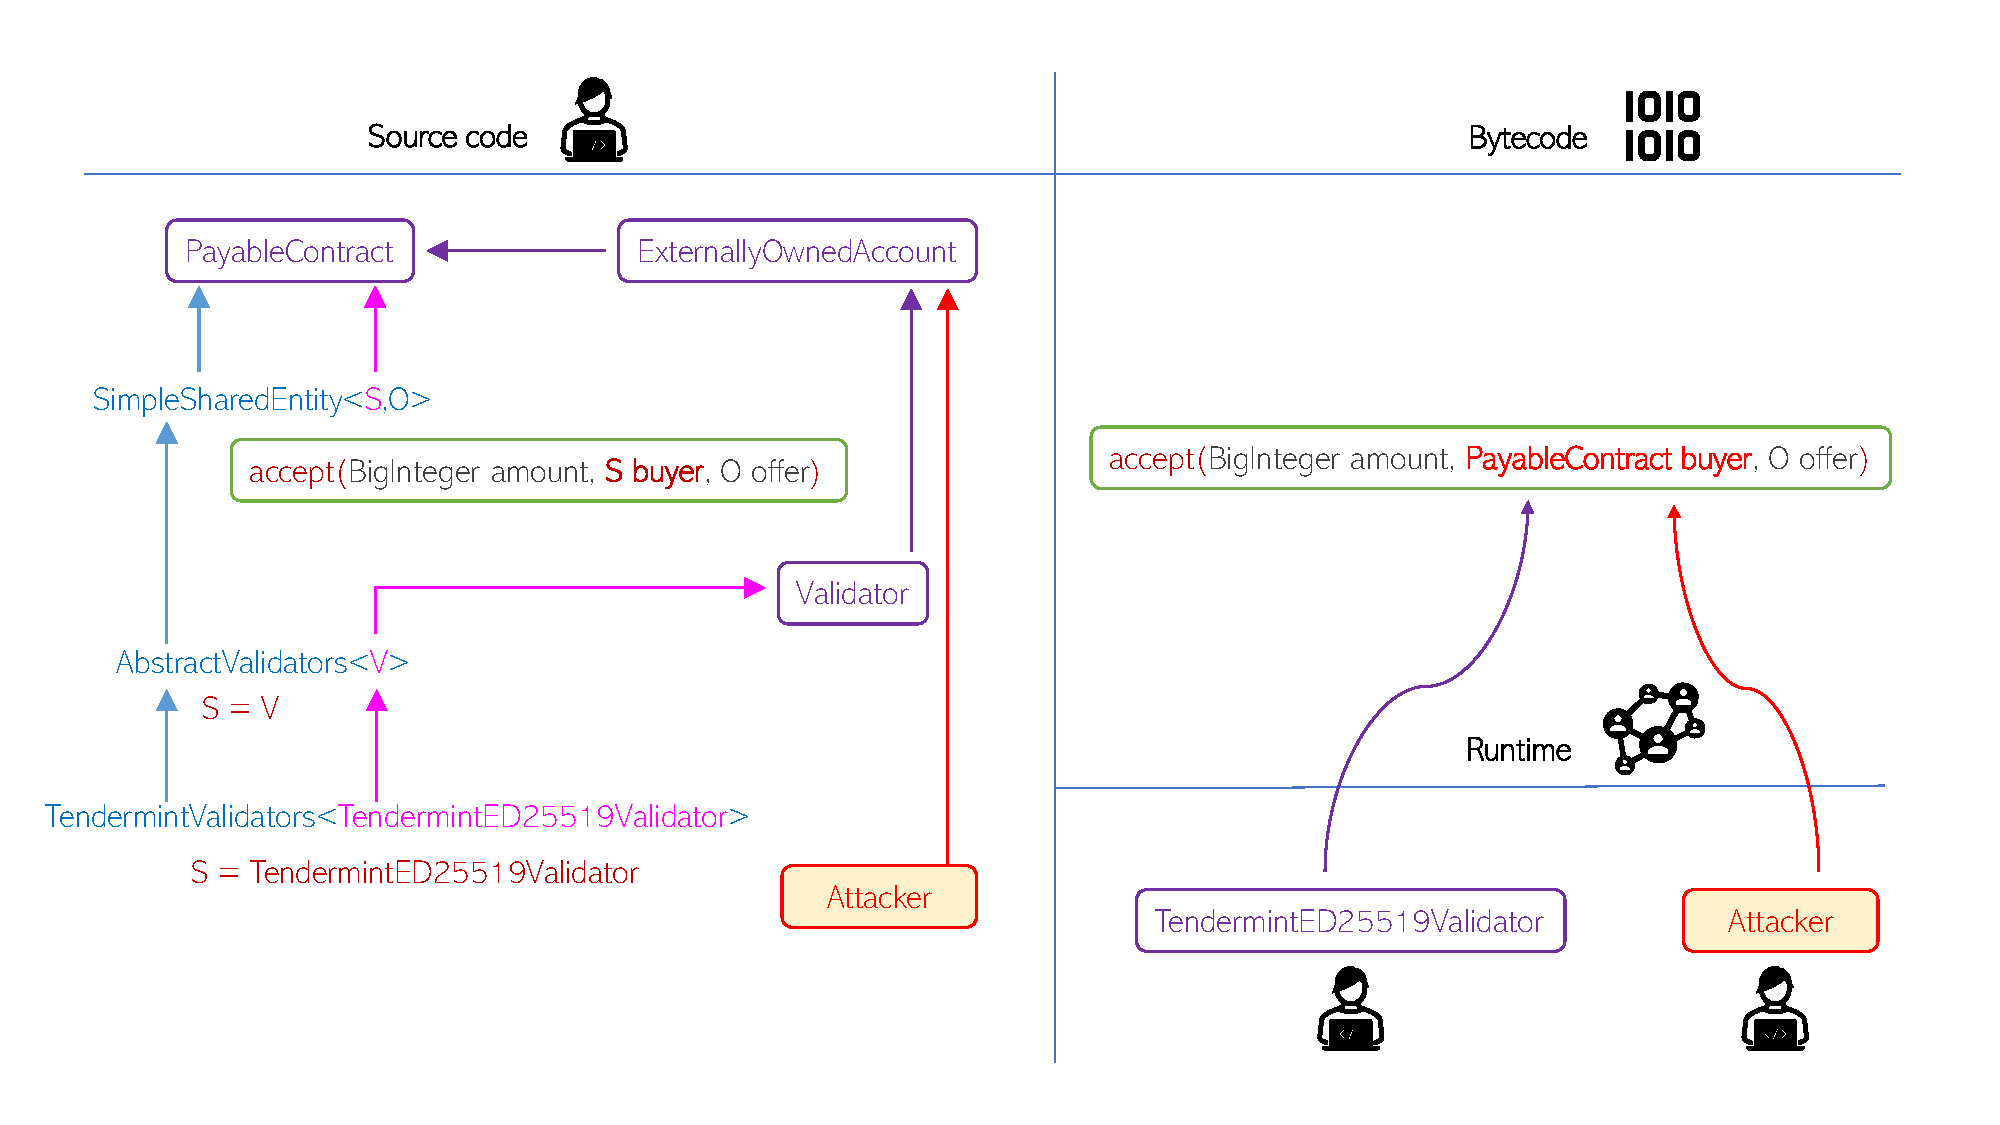
\includegraphics[width=0.9\linewidth]{figures/attack}
\caption{Example of possible attack to a smart contract using Java generics.}
\label{figure.attack}
\end{figure*}

There is, however, a problem with the reasoning
in the previous paragraph. Namely, absence of unchecked
operations guarantees strong typing of Java \emph{source} code. But what is installed
and executed in blockchain is the Java bytecode that has been derived from
the compilation of the code in Fig.~\ref{fig:simple_shared_entity}.
Malicious users might install in blockchain some manually crafted bytecode,
not derived from its Java source code compiled together with the source code
in Fig.~\ref{fig:simple_shared_entity}.
That crafted code might
call the methods of \<SimpleSharedEntity>s in order to attack
that contract. In particular,
the signature of method \<accept> declares a parameter \<buyer> of type \<S> at source code level, but
its compilation into Java bytecode declares an erased
parameter \<buyer> of type \<PayableContract> instead.
It follows that an attacker can install in blockchain a snippet of bytecode that calls
\<accept> and passes \emph{any} \<PayableContract>, not only those that are instances of \<S>:
the \emph{Consistency of Shareholders} property is easily violated at bytecode level.





In particular, it is important that the \emph{Consistency of Shareholders} property holds
for the subclass \<TendermintValidators>: its shareholders
must be \<TendermintED25519Validator>s (as declared in the generic
signature of \<TendermintValidators> in Fig.~\ref{fig:validators}) that enforce a
match between their public key, that identifies who can spend the rewards sent to the validator,
and their Tendermint identifier, that identifies which node of the blockchain
must do the validation work (see how the constructor initializes \<this.id> in
Fig.~\ref{fig:validator}).
If it were possible to add a shareholder of another
type \<Attacker>, the code of \<Attacker> could decouple the node identifier from its
public key (see Fig.~\ref{fig:attacker}):
Tendermint would expect the node (belonging to the \emph{victim}) to do
the validation work while the owner
of the private key of the \<Attacker> could just wait for accrued rewards to spend.
A sort of validator's slavery.
Sec.~\ref{sec:shared_entities} asserted that the \emph{Consistency of Shareholders}
property holds, at source level.
Namely, an \<attacker> (of type \<Attacker>) can only become shareholder
by accepting an ongoing sale \<offer> of shares through a call to
\<tv.accept(offer.cost, attacker, offer)> (Fig.~\ref{fig:simple_shared_entity}).
This is impossible at source level (left part of Fig.~\ref{figure.attack}),
where that call does \emph{not} compile, since \<attacker> has type \<Attacker> that
is not an instance of \<V>, which has been set to \<TendermintED25519Validator>.
But a Hotmoka blockchain contains only the bytecode of \<SimpleSharedEntity>,
where the signature of \<accept> has been erased into
\<accept(BigInteger amount, PayableContract buyer, Offer offer)>
(see Fig.~\ref{figure.java_generics_erasure} and the right part of
Fig.~\ref{figure.attack}).
Hence a blockchain transaction that invokes \<tv.accept(offer.cost, attacker, offer)>
at bytecode level
\emph{does} succeed, since \<attacker> is an externally owned account and all such accounts
are instances of \<PayableContract> (Fig.~\ref{fig:hierarchy-entities}).
That transaction adds \<attacker> to the shareholders of \<tv>,
therefore violating the \emph{Consistency of Shareholders} property and allowing
validator's slavery.
